%%%%%%%%%%%%%%%%%%%%%%%%%%%%%%%%%%%%%%%%%%%%%%%%%%
% Basic setup. Most papers should leave these options alone.
\documentclass[fleqn,usenatbib]{mnras}

\usepackage[T1]{fontenc}
\DeclareRobustCommand{\VAN}[3]{#2}
\let\VANthebibliography\thebibliography
\def\thebibliography{\DeclareRobustCommand{\VAN}[3]{##3}\VANthebibliography}

%%%%% AUTHORS - PLACE YOUR OWN PACKAGES HERE %%%%%
\usepackage{graphicx}	% Including figure files
\usepackage{amsmath}	% Advanced maths commands
\usepackage{amssymb}	% Extra maths symbols
\usepackage{xspace} 
\usepackage{xcolor}
\usepackage{CJK}
\usepackage{fontawesome}
\usepackage{gensymb}
\usepackage{multirow}

%%%%% AUTHORS - PLACE YOUR OWN COMMANDS HERE %%%%%
\newcommand{\ToDo}[1]{\textbf{\textcolor{blue}{ToDo: #1}}}
\newcommand{\LM}[1]{{\textcolor{purple}{LM: #1}}}
\newcommand{\SB}[1]{{\textcolor{orange}{SB: #1}}}
\newcommand{\TB}[1]{{\textcolor{green}{TB: #1}}}

\newcommand{\Gaia}{\textit{Gaia}\xspace} % \Gaia

\usepackage{newtxtext,newtxmath}
%%%%%%%%%%%%%%%%%%%%%%%%%%%%%%%%%%%%%%%%%%%%%%%%%%

%%%%%%%%%%%%%%%%%%% TITLE PAGE %%%%%%%%%%%%%%%%%%%

% Title of the paper, and the short title which is used in the headers.
% Keep the title short and informative.
\title[Accreted stars in NIHAO]{Finding accreted stars in the Milky Way: clues from NIHAO simulations}

% The list of authors, and the short list which is used in the headers.
% If you need two or more lines of authors, add an extra line using \newauthor
\author[L. Mijnarends et al.]{
L. Mijnarends,$^{1}$\thanks{E-mail: u6956623@anu.edu.au}
S. Buder,$^{1,2}$
T. Buck,$^{3}$
\\
% List of institutions
$^{1}$Research School of Astronomy \& Astrophysics, Australian National University, ACT 2611, Australia\\
$^{2}$Center of Excellence for Astrophysics in Three Dimensions (ASTRO-3D), Australia\\
$^{3}$Leibniz-Institut f{\"u}r Astrophysik Potsdam (AIP), An der Sternwarte 16, D-14482 Potsdam, Germany\\
}

% These dates will be filled out by the publisher
\date{Accepted XXX. Received DD MM 2022; in original form DD MM 2022}

% Enter the current year, for the copyright statements etc.
\pubyear{2022}

% Don't change these lines
\begin{document}
\label{firstpage}
\pagerange{\pageref{firstpage}--\pageref{lastpage}}
\maketitle

% Abstract of the paper
\begin{abstract}
%Context: 
Galactic accretion, the merging of the early Milky Way with smaller galaxies, is hypothesised as a plausible explanation for several of the properties of the Milky Way, as we see it today, including old stars on dynamically hot orbits and the bimodality of chemical composition within the stellar disk. Testing this hypothesis and the importance of mergers on the shape of the Milky Way has so far been hindered by our ability to find and characterise accreted stars and their now-dispersed host galaxies.
%Aims: 
We aim to use a cosmological zoom-in simulation from the NIHAO suite, which now also traces the chemical composition of selected elements, to assess accreted stars in a simulated Milky Way analogue and probe ways to distinguish accreted from in-situ stars.
%Method:
By comparison with observations of our Milky Way provided by the stellar spectroscopic GALAH survey, we assess several diagnostic plots in chemical and age-abundance space to identify accreted stars.
%Results:
While we find that the simulations do not reproduce a significant overdensity of accreted stars in the [Al/Fe] vs. [Mg/Mn] plane, we find a promising avenue of identifying accreted stars in stellar age vs. [X/H] diagrams. We thus test the needed precision of ages and abundances (as predicted by the simulation) to separate in-situ and accreted sequences with more than 68\% confidence. We find a significant separation for age and abundance uncertainties below 15\% and $0.2\,\mathrm{dex}$, respectively.
%Conclusions:
Our study predicts that we will be able to better identify and characterise accretion in our Milky Way once we hit an uncertainty threshold. It thus confirms the need for more as well as more precise ages and abundances, as will be delivered by the second phase of the GALAH survey.
%Currently too long! Need to limit to 250 words and 1920 characters...
\end{abstract}

% Select between one and six entries from the list of approved keywords.
% Don't make up new ones.
\begin{keywords}
cosmology: observations -- Galaxy: formation -- Galaxy: evolution -- Galaxy: abundances -- methods: data analysis
\end{keywords}

%%%%%%%%%%%%%%%%%%%%%%%%%%%%%%%%%%%%%%%%%%%%%%%%%%

%%%%%%%%%%%%%%%%% BODY OF PAPER %%%%%%%%%%%%%%%%%%

\section{Introduction}
\label{sec:intro}

The history of the Milky Way is a puzzle that has taunted astronomers for decades. The long lifetimes and unchanging chemical composition of stars makes them a key piece in the puzzle, allowing insights into the historical processes that have led to our Galaxy as we know it today. The advent of new large-scale stellar surveys, providing a wealth of information including measurements of elemental abundances\footnote{We define elemental abundances, such as [Fe/H], [Mg/Fe], and [Mg/Mn] as logarithmic ratios of two elemental number densities compared to the Sun, that is, $\left[\frac{X}{Y}\right]=\log_{10}\left(\frac{N_X}{N_Y}\right) -\log_{10}\left(\frac{N_X}{N_Y}\right)_\odot$.}  for millions of stars has enabled insights into the long and complex history of our Galaxy that have been previously unattainable. The first data release from the \Gaia satellite in 2016 \citep{Brown2016} catalysed a cascade of new discoveries and discussions: a product of the survey’s unprecedented accuracy and scale \citep{BlandHawthorn2019}. \Gaia’s astrometric data complements corresponding advancements in spectroscopic surveys, allowing for significant improvement in our understanding of the chemical makeup of stars \citep{Buck2021}. For example, this study relies on the \textit{GALactic Archaeology with HERMES} (GALAH) survey, based at the Australian-Anglo telescope, which was designed to provide chemical data for up to one million of the stars observed by Gaia \citep{Buder2021}. Using the GALAH data and cosmological simulations to explore the best diagnostic plot with which we can recognise accreted stars in the Milky Way, this report aims to contribute a small piece in our burgeoning understanding of galactic accretion. 

% The history of the Milky Way is a puzzle that has taunted astronomers for decades. Their long lifetimes and unchanging chemical composition through Galactic evolution means that stars in the Milky Way hold key insights to our understanding of the processes that have led to our Galaxy as we know it today. The advent of new large-scale stellar surveys, providing measurements of elemental abundances\footnote{We define elemental abundances, such as [Fe/H], [Mg/Fe], and [Mg/Mn] as logarithmic ratios of two elemental number densities compared to the Sun, that is, $\left[\frac{X}{Y}\right]=\log_{10}\left(\frac{N_X}{N_Y}\right) -\log_{10}\left(\frac{N_X}{N_Y}\right)_\odot$.} for millions of stars has enabled insights into the long and complex history of our Galaxy that have been previously unattainable. When the first data from the \Gaia satellite was released in 2016 \citep{Brown2016}, it catalysed a cascade of new discoveries and discussions: a product of the survey's unprecedented accuracy and scale \citep{BlandHawthorn2019}. \Gaia's astrometric data complements corresponding advancements in spectroscopic surveys that are allowing for significant improvement in our understanding of the chemical makeup of stars \citep{Buck2021}. The \textit{GALactic Archaeology with HERMES} (GALAH) survey\footnote{\url{https://www.galah-survey.org}}, based at the Australian-Anglo telescope, is at the forefront of our improved spectroscopic capabilities \citep{DeSilva2015}. Created to provide chemical data for up to one million of the stars observed by \Gaia, the combined use of \Gaia and GALAH possesses undeniable potential for the field of galactic archaeology, promising to pave the way for improved analysis and understanding of our Galaxy \citep{Buder2021}. This report aims to contribute a small piece in our burgeoning understanding of galactic evolution: combining cosmological simulations and the spectroscopic GALAH data to explore the best option for diagnostic plots with which we can recognise accreted stars in the Milky Way.  

% - difference in the evolution of chemical abundances, both [X/H] and [X/Fe] expected from theoretical predictions of chemical evolution \citep[see e.g.][]{Kobayashi2020}.
% \begin{equation}
% \left[\frac{X}{Y}\right]=\log_{10}\left(\frac{N_X}{N_Y}\right)_{star} -\log_{10}\left(\frac{N_X}{N_Y}\right)_{sun}
% \end{equation}

Interesting papers to keep in mind:
\begin{itemize}
    \item \citet{Martig2021}
    \item \citet{GarciadelaCruz2021, GarciadelaCruz2021b}
    \item \citet{Pinna2019,Pinna2019b}
    \item circularity vs. age \citet{Zhu2022}
\end{itemize}

\subsection{Identifying accreted stars - clues from observations}

% A large array of methods have been used in the search for accreted stars; of which an extensive list can be found in the appendix of \citet{Buder2022}. Here, we refer to the pioneering research by \citet{Nissen2010} which consolidated distinct stellar abundances with previously identified distinct kinematic features. \citet{Belokurov2018} further studied the kinematic distribution in the stellar halo to conclude that the halo was formed by one large accretion event. \citet{Helmi2018} is another notable work that laid the foundations for this letter.  These findings are further outlined by \citet{Naidu2020}, with combinatory use of $L_Z$ vs. $E$, $V_R$ vs. $V_\phi$, $J_\phi/J_\text{tot}$ vs $(J_Z - J_R)/J_\text{tot}$ $R$ vs. $e$, [Fe/H], [Fe/H] vs. [Mg/Fe] etc. to provide evidence of a substructure-dominated halo. \par
% This research uses chemical tagging to identify accreted stars within the Milky Way- a method that has been done in previous studies by \citet{Hawkins2015}, \citet{Das2020} and \citet{Buder2022}. \citet{Martig2021} identify elemental abundance over time in extra-galactic sources as a possible diagnostic tool, which is further explored in this letter. \par 

An extensive list of the wide array of methods that have been used in the search for accreted stars can be found in the appendix of \citet{Buder2022}. Here, we refer to the pioneering research by \citet{Nissen2010}, which consolidated distinct stellar abundances with previously identified distinct kinematic features. \citet{Belokurov2018} and \citet{Helmi2018} further studied the dynamic distribution in the stellar halo, resulting in the discovery of the large accretion event termed the Gaia-Sausage-Enceladus. This finding was further outlined by \citet{Naidu2020}, with combinatory use of $L_Z$ vs. $E$, $V_R$ vs. $V_\phi$, $J_\phi/J_\text{tot}$ vs $(J_Z - J_R)/J_\text{tot}$ $R$ vs. $e$, [Fe/H], [Fe/H] vs. [Mg/Fe] etc. to provide evidence of a substructure-dominated halo. \par
Building upon these works, \citet{Hawkins2015}, \citet{Das2020} and \citet{Buder2022} use chemical tagging to identify accreted stars, outlining a number of potential diagnostic chemical abundance plots, which were used as a foundation for this study. We also draw upon the work of \citet{Martig2021}, which identified plots of elemental abundance over time in extra-galactic sources as a possible diagnostic tool. \par 

These seminal works are all based on observations and are thus hindered by various shortcomings in accuracy. The timespan over which galactic evolution occurs, where in (presumably axisymmetric) asymmetric potential is evolving, is very long. This poses a few problems with the observables used in these existing studies. Variables such as velocities are not conserved over time, and observables like energies are less conserved. Therein lies one of the key advantages of chemical abundances: they are conserved qualities and thus change very little over time. They are, however, not directly observable and difficult to obtain from stellar spectra and any age-inference tool. This is especially the case in metal-poor stars, as we expected accreted stars to be. 
It is prudent to note here that the GALAH data we are working with is particularly difficult to measure in Aluminium abundance, which can be addressed by using the highly-correlated Sodium values instead. The observed stellar ages are even more uncertain- with an average age uncertainty of $33\pm20\%$. We are currently working with a massive age uncertainty range between $30-50\%$. Cosmological simulations, such as those used in this study, carry no age uncertainties and the particular simulation we use here (\citep{Buck2021}) now also includes chemical abundance information. This will provide an exceptional preliminary dataset for exploring potential diagnostic tools, without uncertainty margins to consider. 



% All of these plots that are based on observations are hindered by various issues in accuracy. The timespans over which galactic evolution occurs, wherein the asymmetric potential (assumed to be axisymmetric) is evolving are very long. This means that several observables used in several of the above works are either not conserved (such as velocities) or less conserved (e.g. energies). This can be addressed by using chemical abundances, which are conserved quantities and expected to change very little over time. However, abundances are not directly observable and difficult to obtain from stellar spectra and any age-inference tool. This is especially the case in metal-poor stars, as we expect accreted stars to be.\par 
% It is prudent to note here that the GALAH data we are working with is particularly difficult to measure in Aluminium abundance, which can be addressed by using the highly-correlated Sodium values instead. The observed stellar ages are even more uncertain- with an average age uncertainty of $33\pm20\%$. When  assuming age uncertainties of $30-50\%$, a star’s true age with a measured age of 5Gyr could be anywhere between 2.5 Gyr and 7.5 Gyr old- a massive margin.
% Cosmological zoom-in simulations carry no age uncertainties and the particular simulation we use here (\citep{Buck2021}) now also includes chemical abundance information. 



% We are basically looking for distinct locations of accreted stars with respect to the in-situ stars in whatever observables (or inferred quantities) we can get our hands on. We can simply refer to a summary in appendix of \citet{Buder2022} and just briefly mention here:
% \begin{itemize}
%     \item pioneering studies: \citet{Nissen2010} with [Fe/H] vs. [Mg/Fe] for kinematic halo stars, \citet{Belokurov2018} with $V_R$ vs. $V_\phi$, \citet{Helmi2018} with $L_Z$ vs. $E$; see review: \citet{Helmi2020}
%     \item evidence that halo comprised of substructure: \citet{Naidu2020} with combination of $L_Z$ vs. $E$, $V_R$ vs. $V_\phi$, $J_\phi/J_\text{tot}$ vs $(J_Z - J_R)/J_\text{tot}$ $R$ vs. $e$, [Fe/H], [Fe/H] vs. [Mg/Fe]
%     \item how to identify accreted stars in chemical space: \citet{Hawkins2015, Das2020, Buder2022}, e.g. [Al/Fe] vs. [Mg/Mn] or [Na/Fe] vs. [Mg/Mn]
%     \item extra-galactic studies use age-abundance trends, e.g. \citet{Martig2021}
% \end{itemize}

% Problem: All of these plots from observations have shortcomings: 1) several observables are not conserved (e.g. velocities) or less conserved (e.g. energies) over a longer time-frame and when the asymmetric potential (assumed to be axisymmetric) is evolving. Chemical abundances and ages are much more conserved properties of stars, but 1) not directly observables and 2) hard to obtain from stellar spectra and any kind of age-inference tool - especially for metal-poor stars, as we expect accreted stars to be. Just briefly mention: Al hard to measure for GALAH (can use highly-correlated Na however) and stellar ages also uncertain. The average age uncertainty of stars in GALAH is $33 \pm 20\%$. For main-sequence turn-off stars, the ages are more certain, whereas for giant stars they are on average $42 \pm 15\%$. When assuming age uncertainties of 30-50\%, the true age of a star with a measured age of 5Gyr could be anywhere between 2.5 Gyr and 7.5 Gyr old- a massive margin.

% Cosmological zoom-in simulation have no age uncertainties and now also trace chemical evolution, in particular the simulation that we use here \citep{Buck2021}, a follow-up of the NIHAO simulation suite.

\subsection{NIHAO Zoom-in simulation with chemistry}

The \textit{Numerical Investigation of a Hundred Astronomical Objects} (NIHAO) simulation suite describes a series of 100 “zoom-in” simulations- the most accurate and unbiased galactic models to-date \citep{Wang2015}. In this study, we use a follow-up simulation from NIHAO, produced by \citet{Buck2021}. These simulations use observational data to first fit a chemical evolution model for initial conditions, before being fit to hydrodynamical simulations. The accuracy of the models relies heavily on sufficient observational data, which further reinforces the important of large, accurate surveys like \Gaia and GALAH. The simulations are used throughout this report to compare results from the observational data of GALAH (eg. \citep{Buder2022}, \citep{Hawkins2015}, \citep{Das2020}, as well as introducing evidence to support additional diagnostic plots, such as element-age plots (eg. \citep{Martig2021}).
\par 
The simulation data is available for a selected number of elements of which only ten correspond with the GALAH data. The only elements we are able to work with in both datasets are C, O, Mg, Al, Si, V, Cr, Mn, Co and Ba. For each of these, Fig.~\ref{fig:FeH_XFe} shows the element’s abundance ratio to Hydrogen plotted against [Fe/H], or the metallicity. 

% In this study, we use a follow-up zoom-in simulation from the \textit{Numerical Investigation of a Hundred Astronomical Objects} (NIHAO) simulation suite. NIHAO describes a series of 100 “zoom-in” simulations, the most accurate and unbiased galactic models to-date \citep{Wang2015}. These simulations are characterised as time-resolved chemical enrichment models, where spectral data is taken at specific time intervals, rather than averaged over time. This allows for unprecedented flexibility in the initial parameters and consequently unprecedented accuracy in the models \citep{Buck2021}. 
% More importantly, the simulations by \citet{Buck2021} incorporate a “hybrid approach” wherein observational data is first used to fit a chemical evolution model for initial conditions, before being fit to hydrodynamical simulations \citep{Buck2021}. It is clear therefore that the accuracy of models relies heavily on sufficient observational data \citep{Wang2015}, which reinforces the importance of large, accurate surveys like \Gaia and GALAH. The simulations are used throughout this project to compare to results from the observational data of GALAH, as well as providing an argument for different plots to be used. This allows an unprecedented comparison of accurate measurements with uncertainties and model predictions without uncertainties.

\LM{Motivation for this study: In \citet{Buck2021}, the main focus of the paper was to present the chemical evolution implementation and only a few verification plots have been done, focusing on the stellar disk.}

% The simulation data is available for the elements H, He, C, N, O, Ne, Mg, Al, Si, P, S, V, Cr, Mn, Fe, Co, Ba. Of these, only ten correspond with the GALAH data leaving plots possible for only C, O, Mg, Al, Si, V, Cr, Mn, Co and Ba. For each of these ten, a plot was produced in Python of the element's abundance ratio to Hydrogen, against the abundance ratio [Fe/H], or metallicity. The results of this are shown in Fig.~\ref{fig:FeH_XFe}.

\SB{Question to discuss: Should we renormalise the [X/H] for the elements so that the solar neighborhood lands at 0, as would be custom by definition?}

\subsection{Aims of Study} 

The main aim of this project is to identify the most suitable plot for identifying accreted structures in the Milky Way. This assessment will be based on our ability to observe clear spectral patterns and trends, as well as the clarity of the plots: quantifying the distinction between populations with Gaussian methods. Based on our understanding of how the elements themselves are produced, we can recognise abundance patterns that are different to those that would be produced through the evolution of the Milky Way and thus must be accreted. We assess a range of elements for this purpose, as there is observed overlap between in situ and accreted abundances of some elements, for example Fe.  Analysing the cosmological simulations will assist in this determination, in confirming the origin of the accreted stars selected via chemical tagging, and thus confirming the methodology.

An improved understanding of accretion within the Milky Way encompasses more accurate stellar ages \citep{Das2020}, merger history \citep{Naidu2020}, stellar formation history and chemical enrichment \citep{DeSilva2015}: all facets which contribute to a more accurate picture of our early Universe and its origins. We are entering an exciting period in the field of galactic archaeology and with more and more increasingly accurate data coming out, we are facing the possibility of unprecedented understanding of the Milky Way’s, and the Universe’s, long and complex history.

%%%%%%%%%%%%%%%%%%%%%%%%%%%%%%%%%%%%%%%%%%%%%%%%%%

\section{Diagnostic plots: Observation vs. Simulation}
\label{sec:comparison}

In Sec.~\ref{sec:intro}, we have identified several observation-based plots that have been used to identify accreted stars in the Milky Way. In this section, we are now concerned with replicating these plots for the simulated Milky Way analogue to first order\footnote{\SB{Come back to this if we figure out that we actually do have to limit the simulation space to the Solar neighborhood - which we have not done yet!}}. For this particular study, we will limit ourselves to the following plots: a) [Fe/H] vs. [Mg/Fe] \citep{Nissen2010}, [Al/Fe] vs. [Mg/Mn] \citep{Hawkins2015, Das2020}.

\subsection{Abundance trends: [Fe/H] vs. [X/Fe]} \label{sec:feh_xfe}

There are only ten elements available in both the GALAH dataset and the NIHAO simulations- the abundances of which were plotted against metallicity [Fe/H] in Figure \ref{fig:FeH_XFe}, which highlights the huge divergence between the two. Where clear overdensities can be observed in the observations, there is little distinct substructure in the simulation-based plots, and it is impossible to identify different stellar populations. One of the key advantages to using simulations is the complete lack of corresponding measurement uncertainties. We would expect the substructure to appear even more clearly in the simulations than in the observations, and the fact that this isn’t the case indicates a larger problem in the process.

\begin{itemize}
    %\item Trends for 10 overlapping elements in Fig.~\ref{fig:FeH_XFe}.
    \item To discuss: [C/Fe] and [Ba/Fe] with significant differences!
    \item Then closer look at contributions from SNII vs. SNIa as suggested by \citet{Nissen2010} in Fig.~\ref{fig:low_alpha_halo}. Discuss selection of white polygon and how it does not show a significant overdensity in the [Al/Fe] vs. [Mn/Mn] plot (which could be expected without measurement uncertainties).
    \item Look more generally at the abundance-abundance plots used to identify accreted stars in Sec.~\ref{sec:alfe_mgmn}.
    \item \SB{[Fe/H] vs. [C+N/Fe] \citep{Hawkins2015}?}
\end{itemize}

\begin{figure*}
	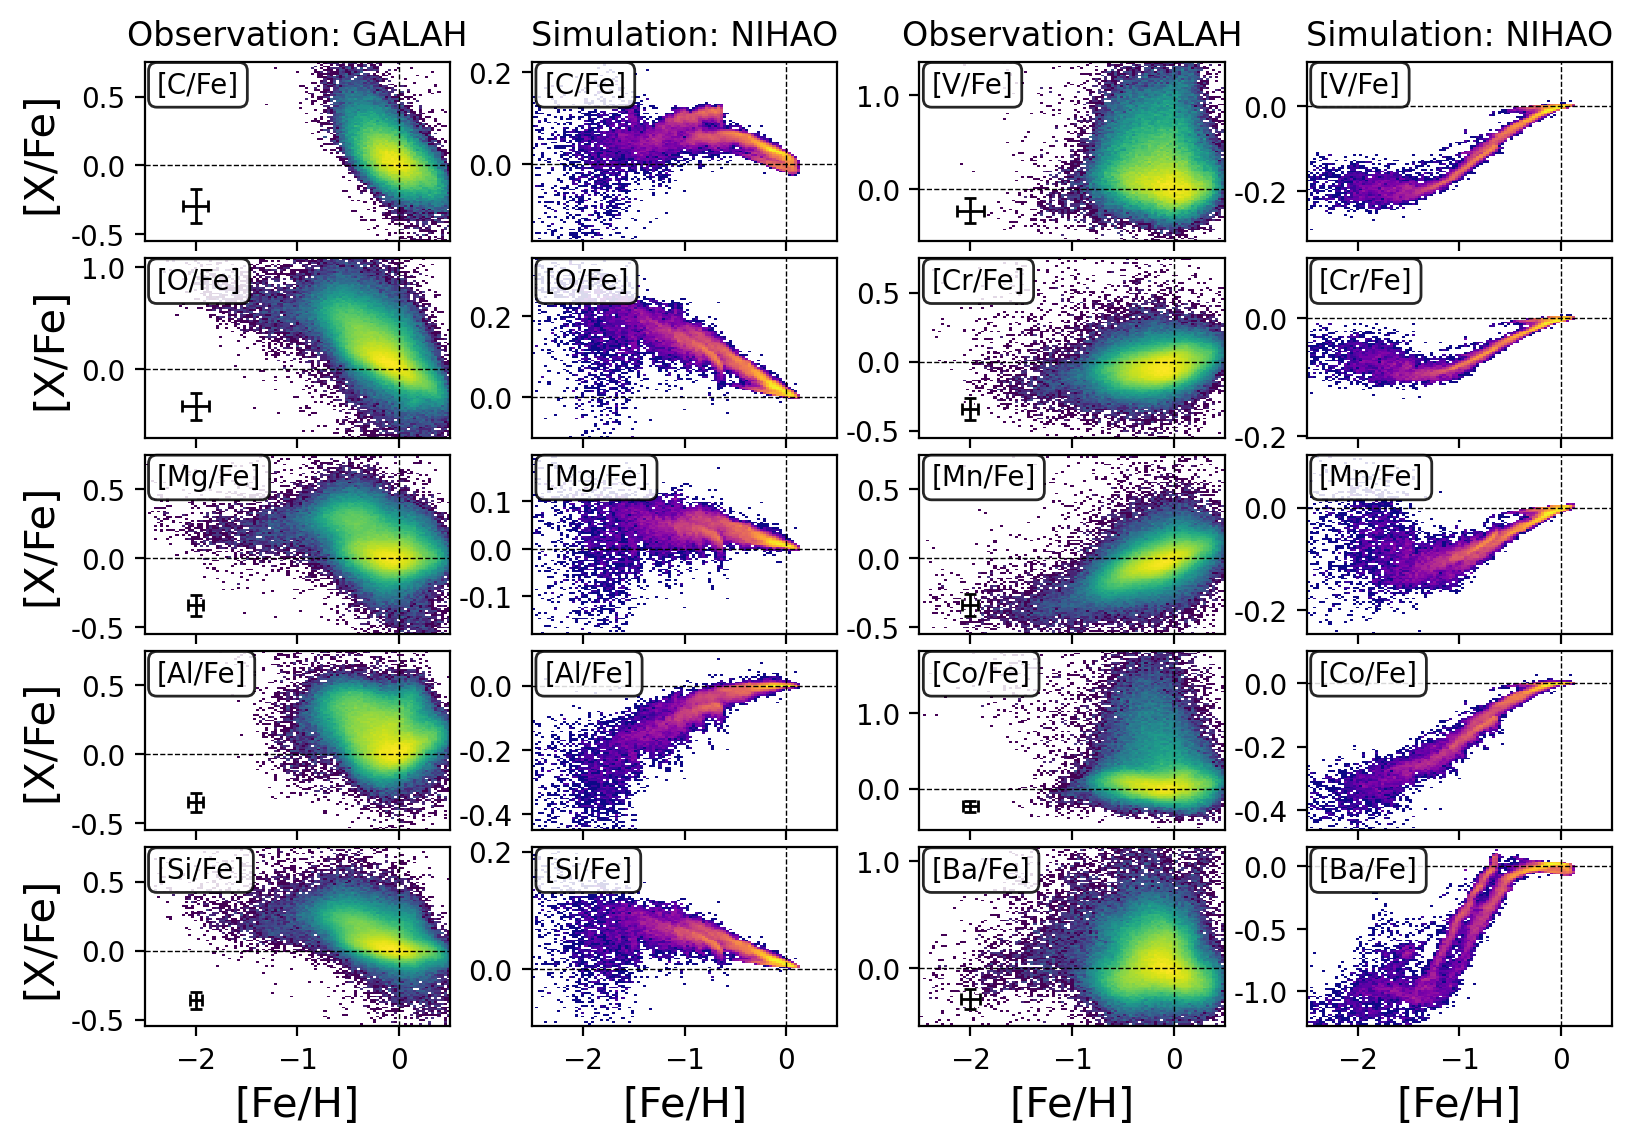
\includegraphics[width=\textwidth]{figures/Overview_FeH_XFe_Obs_Sim.png}
    \caption{
    \textbf{Distribution of elemental abundances [X/Fe] versus [Fe/H] for the ten elements overlapping between GALAH and NIHAO.} 
    \textbf{First and third rows} show observed data from GALAH and \textbf{second and fourth rows} show the simulated data for the same abundance ratios. Color maps are showing the logarithmic density distributions with brightest colors indicating highest densities. For better visibility, plot ranges are adjusted to the data rather than to be equal among each panel. Dashed lines indicate Solar values.}
    \label{fig:FeH_XFe}
\end{figure*}

\begin{figure*}
	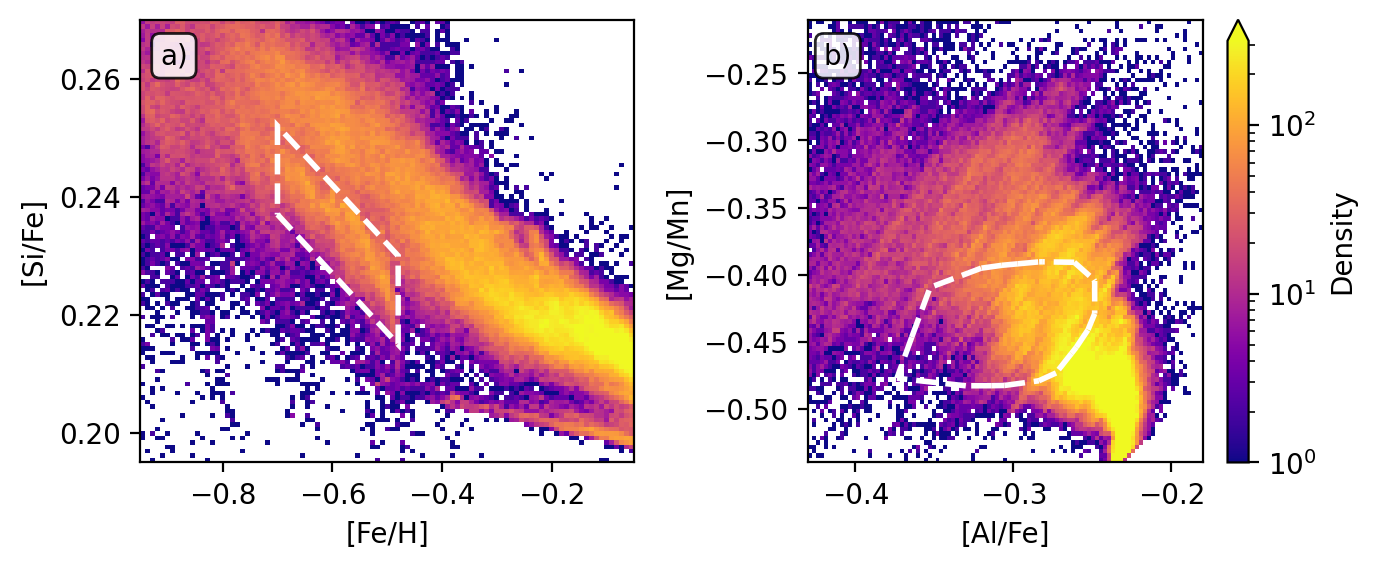
\includegraphics[width=\textwidth]{figures/low_alpha_halo.png}
    \caption{
    \textbf{Chemical abundances for all particles of the simulation (color-coded by logarithmic density) and a subset of particles (selected via white polygon in left plot).} 
    \textbf{Panel a):} iron vs. silicon abundances as tracers of contribution from SNIa and SNII. \textbf{Panel b):} abundance combination [Al/Fe] vs. [Mg/Mn] used to trace accreted stars in observations. A convex hull is used to plot the area of the stars selected via a polygon in panel a).}
    \label{fig:low_alpha_halo}
\end{figure*}

% The first plots produced and analysed were [X/Fe] against [Fe/H], from both the observation and simulation data, which allowed for a side-by-side comparison to be made. [Fe/H] is generally representative of the metallicity of a star, which has significant implications for its age and the ISM from which it was born, which is why [Fe/H] is used often as a basis over which to plot a range of elemental abundances \citep{Buder2022}.  

% This abundance plane has been plotted many times throughout the existing literature and has consistently produced a clear distinction in substructure from measured spectra \citep{Das2020, Nissen2010}. When these plots were reproduced for this report, as in Fig.~\ref{fig:allvsFeH}, in the observation-based plots (right), there are clear overdensities observed, separate to the main, in situ population. When compared to the simulations (left) however, there is very little distinct substructure to be noted. There is significant overlap in the chemical abundance planes in the simulation data, resulting in no clear substructure and making it impossible to identify in situ or accreted stars from the plots.  
% One of the key advantages to using simulations is the complete lack of corresponding measurement uncertainties. We would expect the substructure to appear even more clearly in the simulations than in the observations, and the fact that this isn't the case indicates a larger problem in the process. 

\subsection{Abundance-abundance plots: [Al/Fe] vs. [Mg/Mn]} \label{sec:alfe_mgmn}

We then plot the ratio of a light odd-z element (Na and Al) against alpha element Mg over Mn, shown in Figure 3. The ratio of [Mg/Mn] represents the ratio of SNII and SNIa dominated elements respectively. Looking first at the observations, there are clear overdensities visible in both plots.  Both [Na/Fe] and [Al/Fe] plots show the overdensity for the thin/low-alpha disk at the expected solar abundances at (0,0). The high-alpha disk is seen in an overdensity at around (0.4,0.5). More importantly, although not clear for [Al/Fe] with the GALAH data in this report, accreted stars are visible in the [Na/Fe] plot at around (-0.4,0.4). These observations concur with \citet{Das2020} and \citet{Horta2020}, which both used APOGEE data and the [Al/Fe] ratio instead. \par 
In the simulations, there is very significant zeropoint shift from the observations, where the only clear overdensity of the thin disk is at (-0.23, -0.55) instead of the expected (0,0). The overall shape and structural composition is also massively different from the plots created with GALAH data. The simulations contain zero noise, and it was expected that this would clarify the results seen in the observational data. The fact that this was not the case may indicate different chemical evolution in the simulation and the actual Milky Way. This could be either because they are truly inherently different or the result of inaccurate chemical enrichment in the simulation. 



% \begin{itemize}
%     \item As suggested by \citet{Hawkins2015} and \citet{Das2020} based on data from the APOGEE survey as well as \citet{Buder2022} based on data from the GALAH survey, we plot the ratio of a light odd-Z element (Na and Al) as well as the ratio of SNII and SNIa dominated elements (Mg and Mn, respectively) in Fig.~\ref{fig:alfe_mgmn}.
%     \item Describe observations: overdensities for thin/low-alpha disk around (0,0), thick/high-alpha disk at (0.4,0.5) and accreted stars around (-0.4,0.4), refer to \citet{Das2020, Horta2021}. Not so clear for [Al/Fe] with GALAH, but clearer when using [Na/Fe] \citep{Buder2022}. \SB{We could use APOGEE DR17 for a better/clearer comparison.}
%     \item Describe simulations: Zeropoint shift, that is the location of the thin disk around (-0.23,-0.55) instead (0,0). But also overall structure is significantly different: No noise, but also no clear substructure!
%     \item Interpretation: different chemical evolution in simulation and Milky Way (either because truly different or because chemical enrichment in simulation not accurate).
% \end{itemize}

\begin{figure*}
	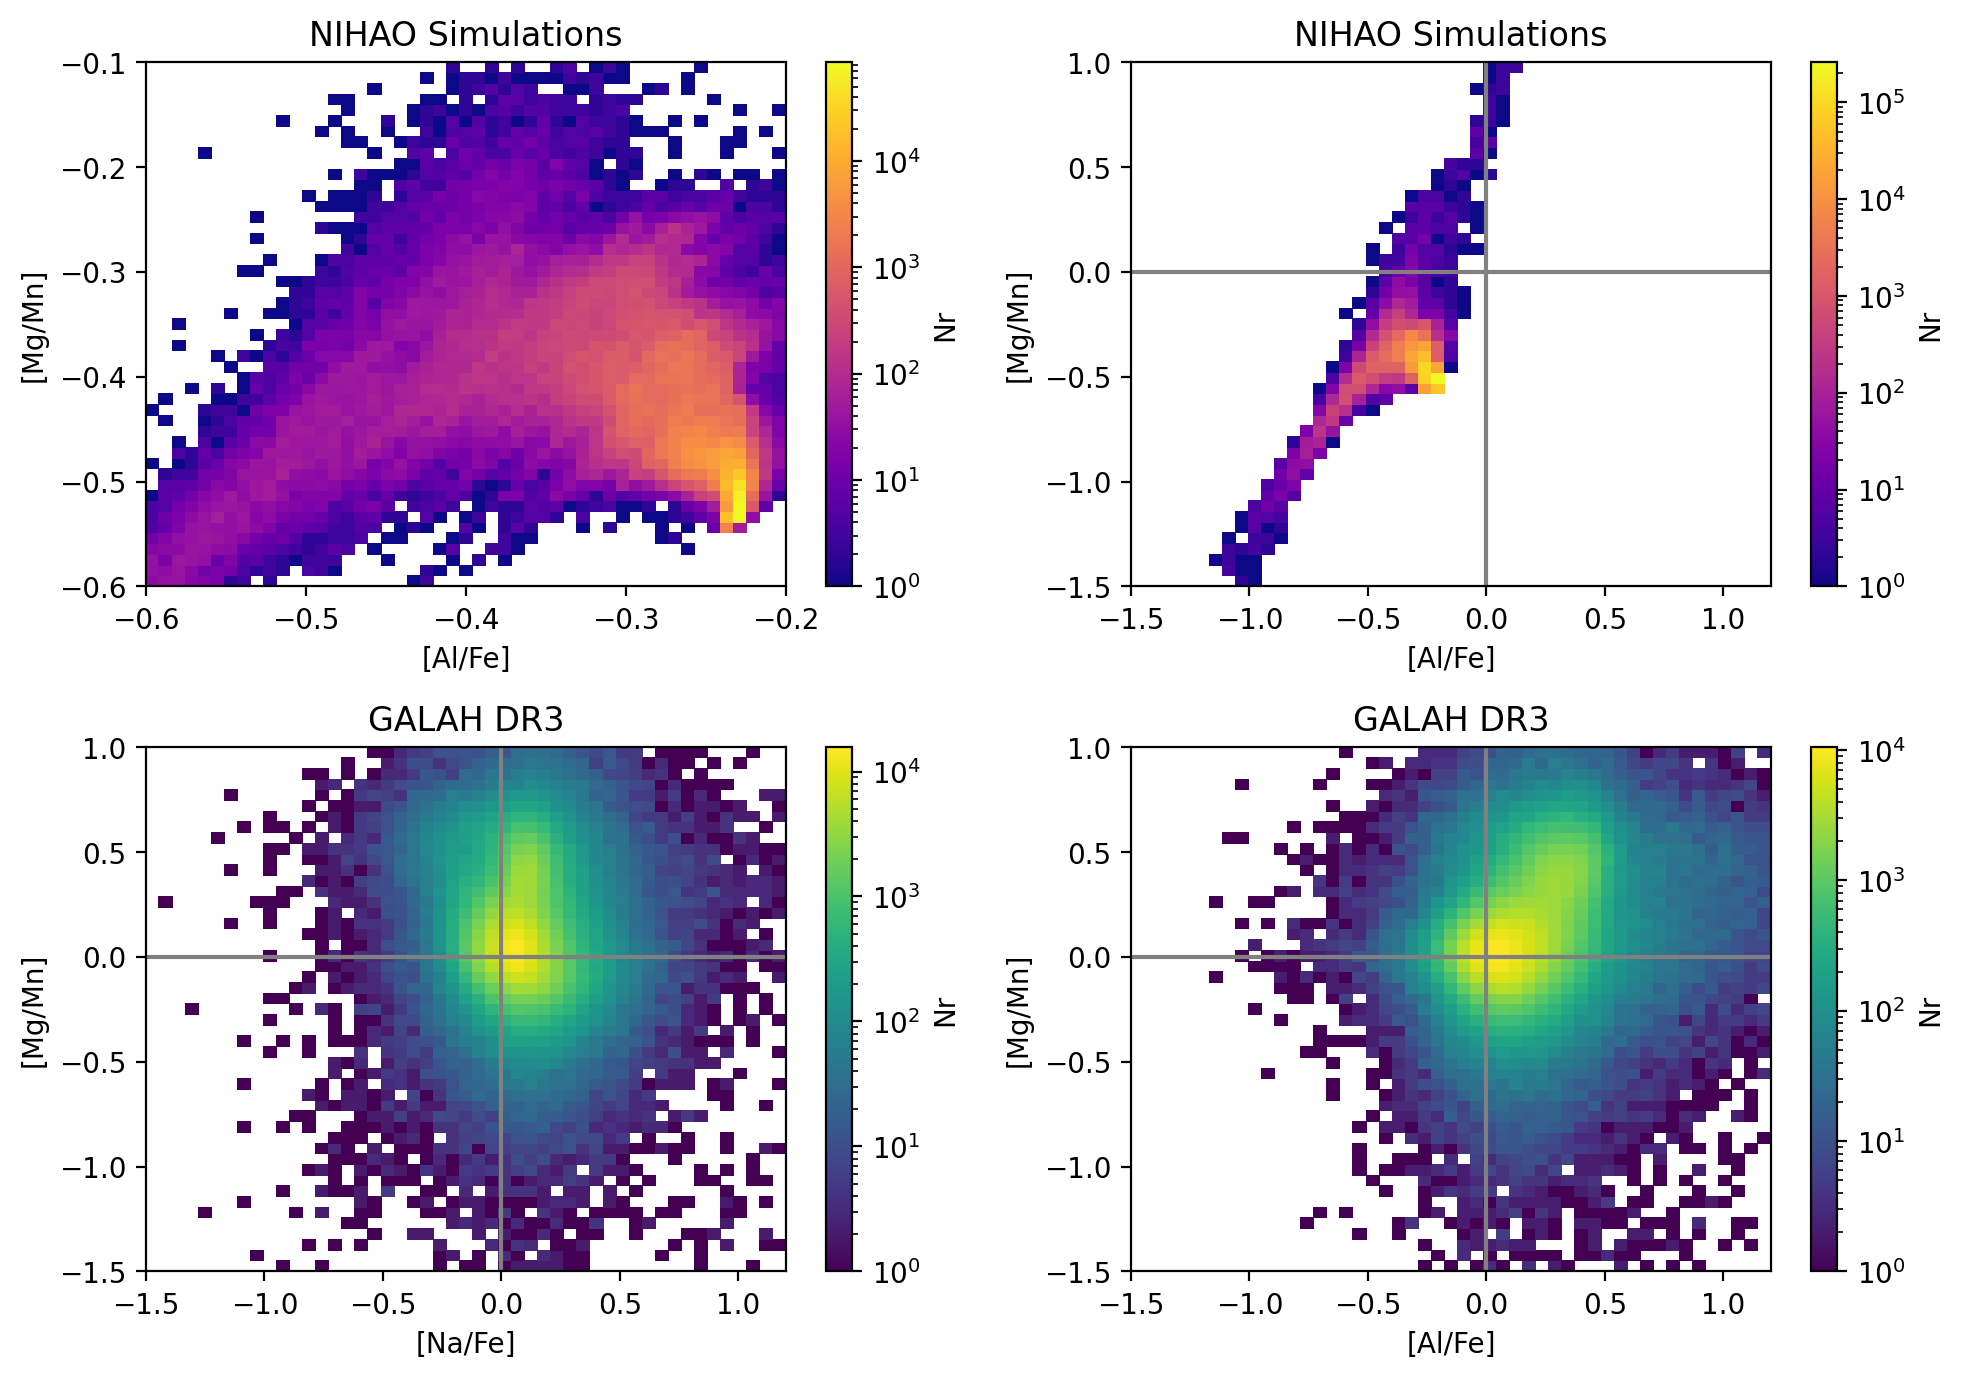
\includegraphics[width=\textwidth]{figures/[MgMn] vs [AlFe].png}
    \caption{Simulation (left) vs observation (right) of alpha element Mg against Mn, plotted over [Al/Fe]. The two plots are on separate axes as the observational plot had to be zoomed in significantly to show any sufficient detail. The zeropoints are completely different, with the axes representing the solar abundances at [0,0] not visible on the observational plot. 
    }
    \label{fig:alfe_mgmn}
\end{figure*}

\section{A new angle: age-abundance-distributions}

Fortunately, chemistry is not the only conserved property of stars. We therefore turn to stellar ages and assess age-abundance trends in the simulations. Observations still suffer from incredibly large uncertainties on the order of $30-50\%$ for most stars, so examining simulation plots remove this barrier and allow to determine chemical enrichment as a function of age, by subtracting the simulated formation age tform from 14.14 Gyr, the age of the simulated universe \citep{Buck2021}. Although the observational plots showed incomprehensible results, there is very clear substructure in the simulated age-abundance plots, with two distinct streams for the two populations (in-situ and accreted).\par 

Accreted populations tend to join the Milky Way from smaller galaxies with less massive stars. This means that the stars are less metal-heavy and explains the lower stream of accreted stars that can be observed in the simulation data. \par 

The stark difference in clarity of results between the uncertainty-free simulation data and the high-uncertainty GALAH data highlights the importance of reducing observation noise, and provides clear motivation for further investigation into these plots as diagnostic tools. Similar plots have been used already with GALAH data to identify accreted substructure in galaxies other than the Milky Way \citep{Martig2021}. 
% \begin{itemize}
%     \item Chemistry is not the only conserved property of stars.
%     \item We therefore turn to stellar ages and assess age-abundance trends in the simulations. This is an especially informative exercise, as stellar ages are currently still suffering from low precisions on the order of 30-50\% for most stars. Our simulation, however, traces the formation age \texttt{tform} as a perfect value and we can infer stellar ages by subtracting \texttt{tform} from the age of the universe, which is $14.14\,\mathrm{Gyr}$ in the simulation.
%     \item Such plots have been used in observed data of other galaxies to identify accreted stars \citep{Martig2021}.
% \end{itemize}
\begin{figure}
	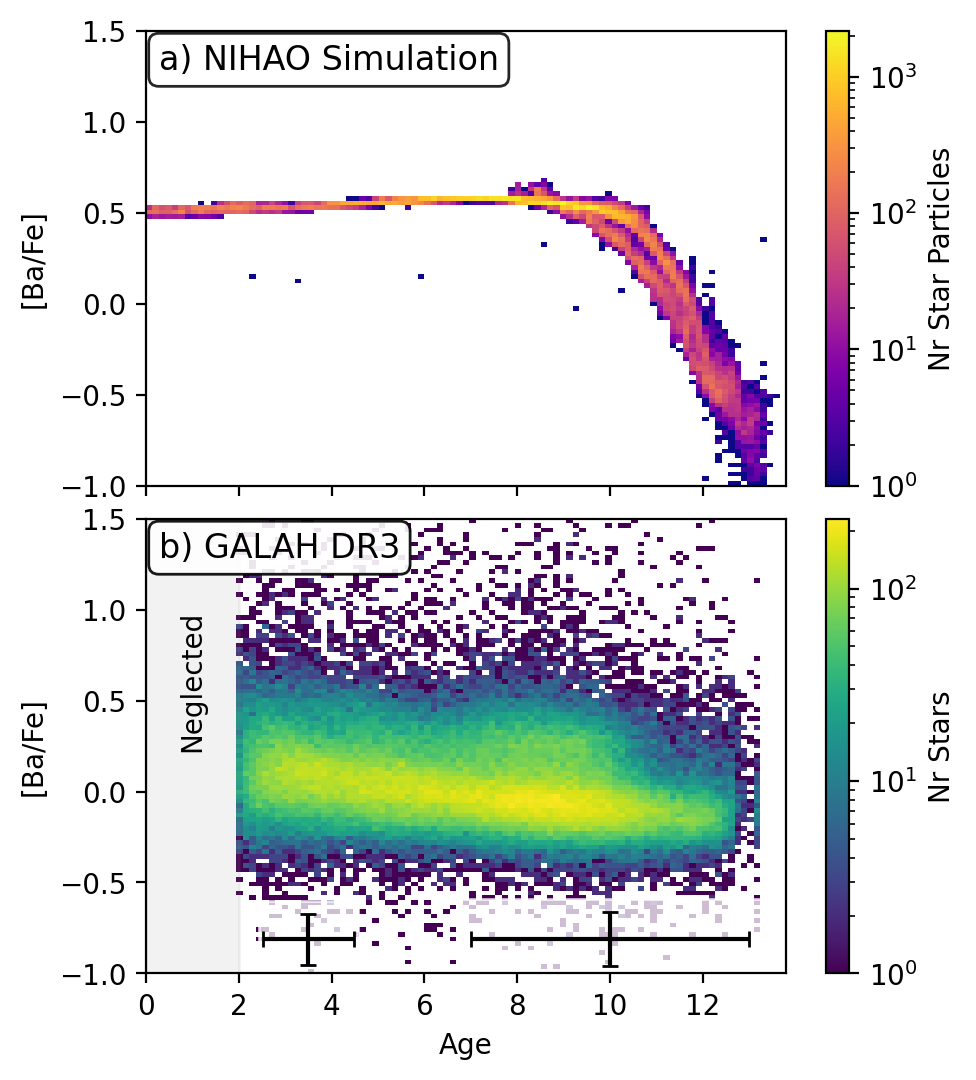
\includegraphics[width=\columnwidth]{figures/Ba_Fe_time.png}
    \caption{Barium abundance in a ratio with Iron [Ba/Fe] as a function of age. Simulation data (top) and GALAH data (bottom) shows clear differences in scatter. Although not entirely separate, it is clear that there are two different overdensities in a 'stream'-like shape.}
    \label{fig:BaFetime}
\end{figure}
\begin{figure}
	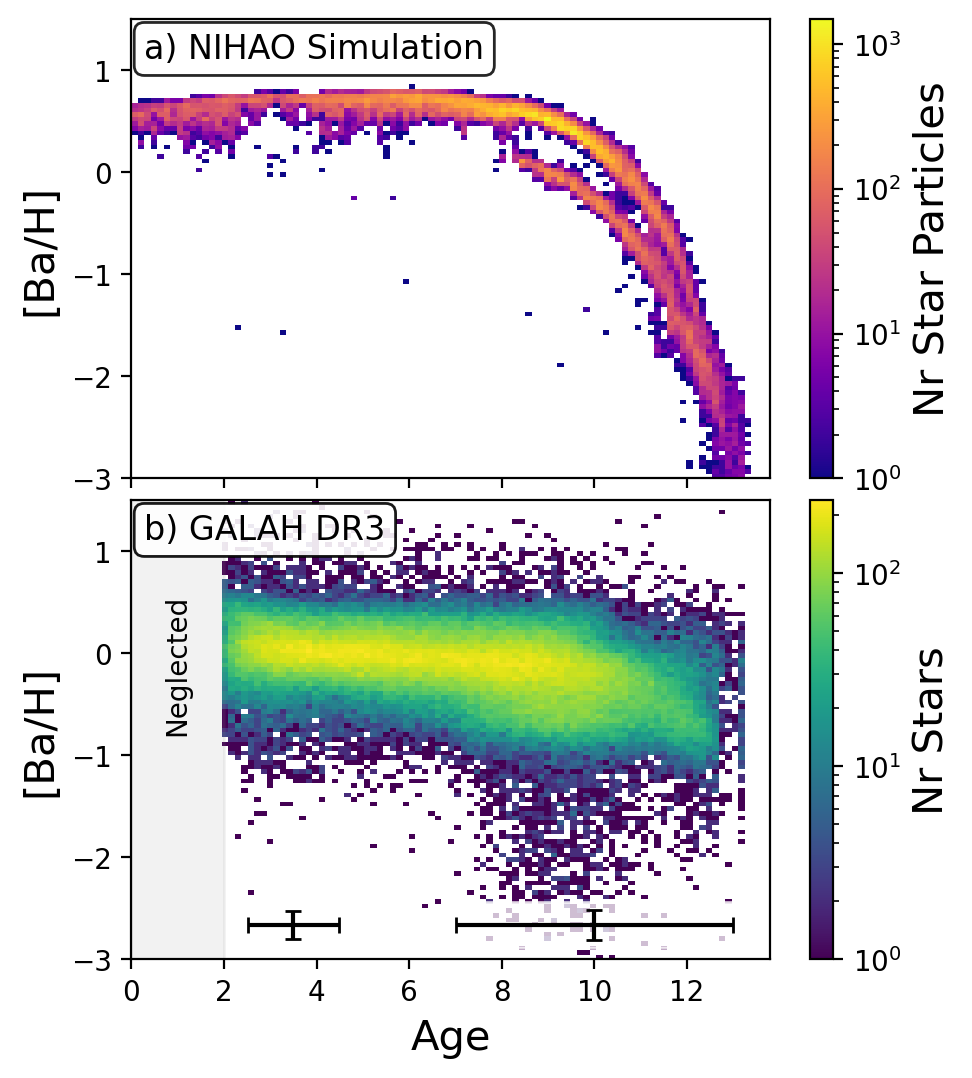
\includegraphics[width=\columnwidth]{figures/Ba_H_time.png}
    \caption{Simulation (top) vs observation (bottom) plots of Barium's evolution with age, with Ba plotted in a ratio against H instead of Fe. The top stream represents the in situ stars, while the lower stream is stars that have since accreted and hence follow a similar evolution path but at lower element abundances.}
    \label{fig:BaHtime}
\end{figure}

\subsection{The importance of notation: [X/Fe] or [X/H]}

\begin{itemize}
    \item Discuss that some previous studies have suggested to use elemental abundances reported as a function of hydrogen number density \citep[see e.g.][]{Fuhrmann2017b, Feuillet2021}.
\end{itemize}

Fig.~\ref{fig:BaHtime} shows the elemental ratio of [Ba/Fe] over time. This same plot was created using every elemental combination available in the dataset, and it was found that the combination of [X/H] over time produced the clearest plot, as in Fig.~\ref{fig:BaHtime}. Hydrogen, being formed in the Big Bang nucleosynthesis, is not enhanced or affected by time, whereas metals like Fe are. This is why [X/H] plots are decidedly clearer than [X/Fe], as Fe is being simultaneously enriched along with Ba.

As the abundances show clear sequences in [Ba/H] (and the other abundances), we now want to study how much noise we could allow for both abundance and age estimates, to still be able to separate the sequences.

\subsection{Quantifying differences of age-abundance sequences} \label{sec:ageabundance}

To quantify the separation significance $r$, we use Eq.~\ref{eq:r_value}, adapted from \citet{Lindegren2013}, to quantify the separation between two sequences, for which we assume a Gaussian distribution around a mean value $\mu$ with a standard deviation $\sigma$:
\begin{equation} \label{eq:r_value}
r = \frac{|\mu_1 - \mu_2|}{\sqrt{\sigma_1^2 + \sigma_2^2}}
\end{equation}

While in the simulation the latter would only incorporate the intrinsic scatter, that is, $\sigma_{1,\text{obs}} = \sigma_1$, the observational scatter (which we assume uniform throughout the parameter space) of actual observations would enter into this equation via
\begin{equation} \label{eq:scatter}
    \sigma_{1,\text{obs}} = \sqrt{\sigma_1^2+\sigma_{obs}^2},
\end{equation}
leading to a slightly adjusted version of Eq.~\ref{eq:r_value}, that is,
\begin{equation} \label{eq:r_value_observed}
r (\sigma_{obs}) = \frac{|\mu_1 - \mu_2|}{\sqrt{\sigma_1^2 + \sigma_2^2 + 2\cdot \sigma_{obs}^2}}.
\end{equation}

We confirm our assumption of Gaussian distributions for the sequences by looking at the histograms of [Ba/H] for the simulation between 8 and $9\,\mathrm{Gyr}$ in Fig.~\ref{fig:hist_labels}.

\begin{figure}
	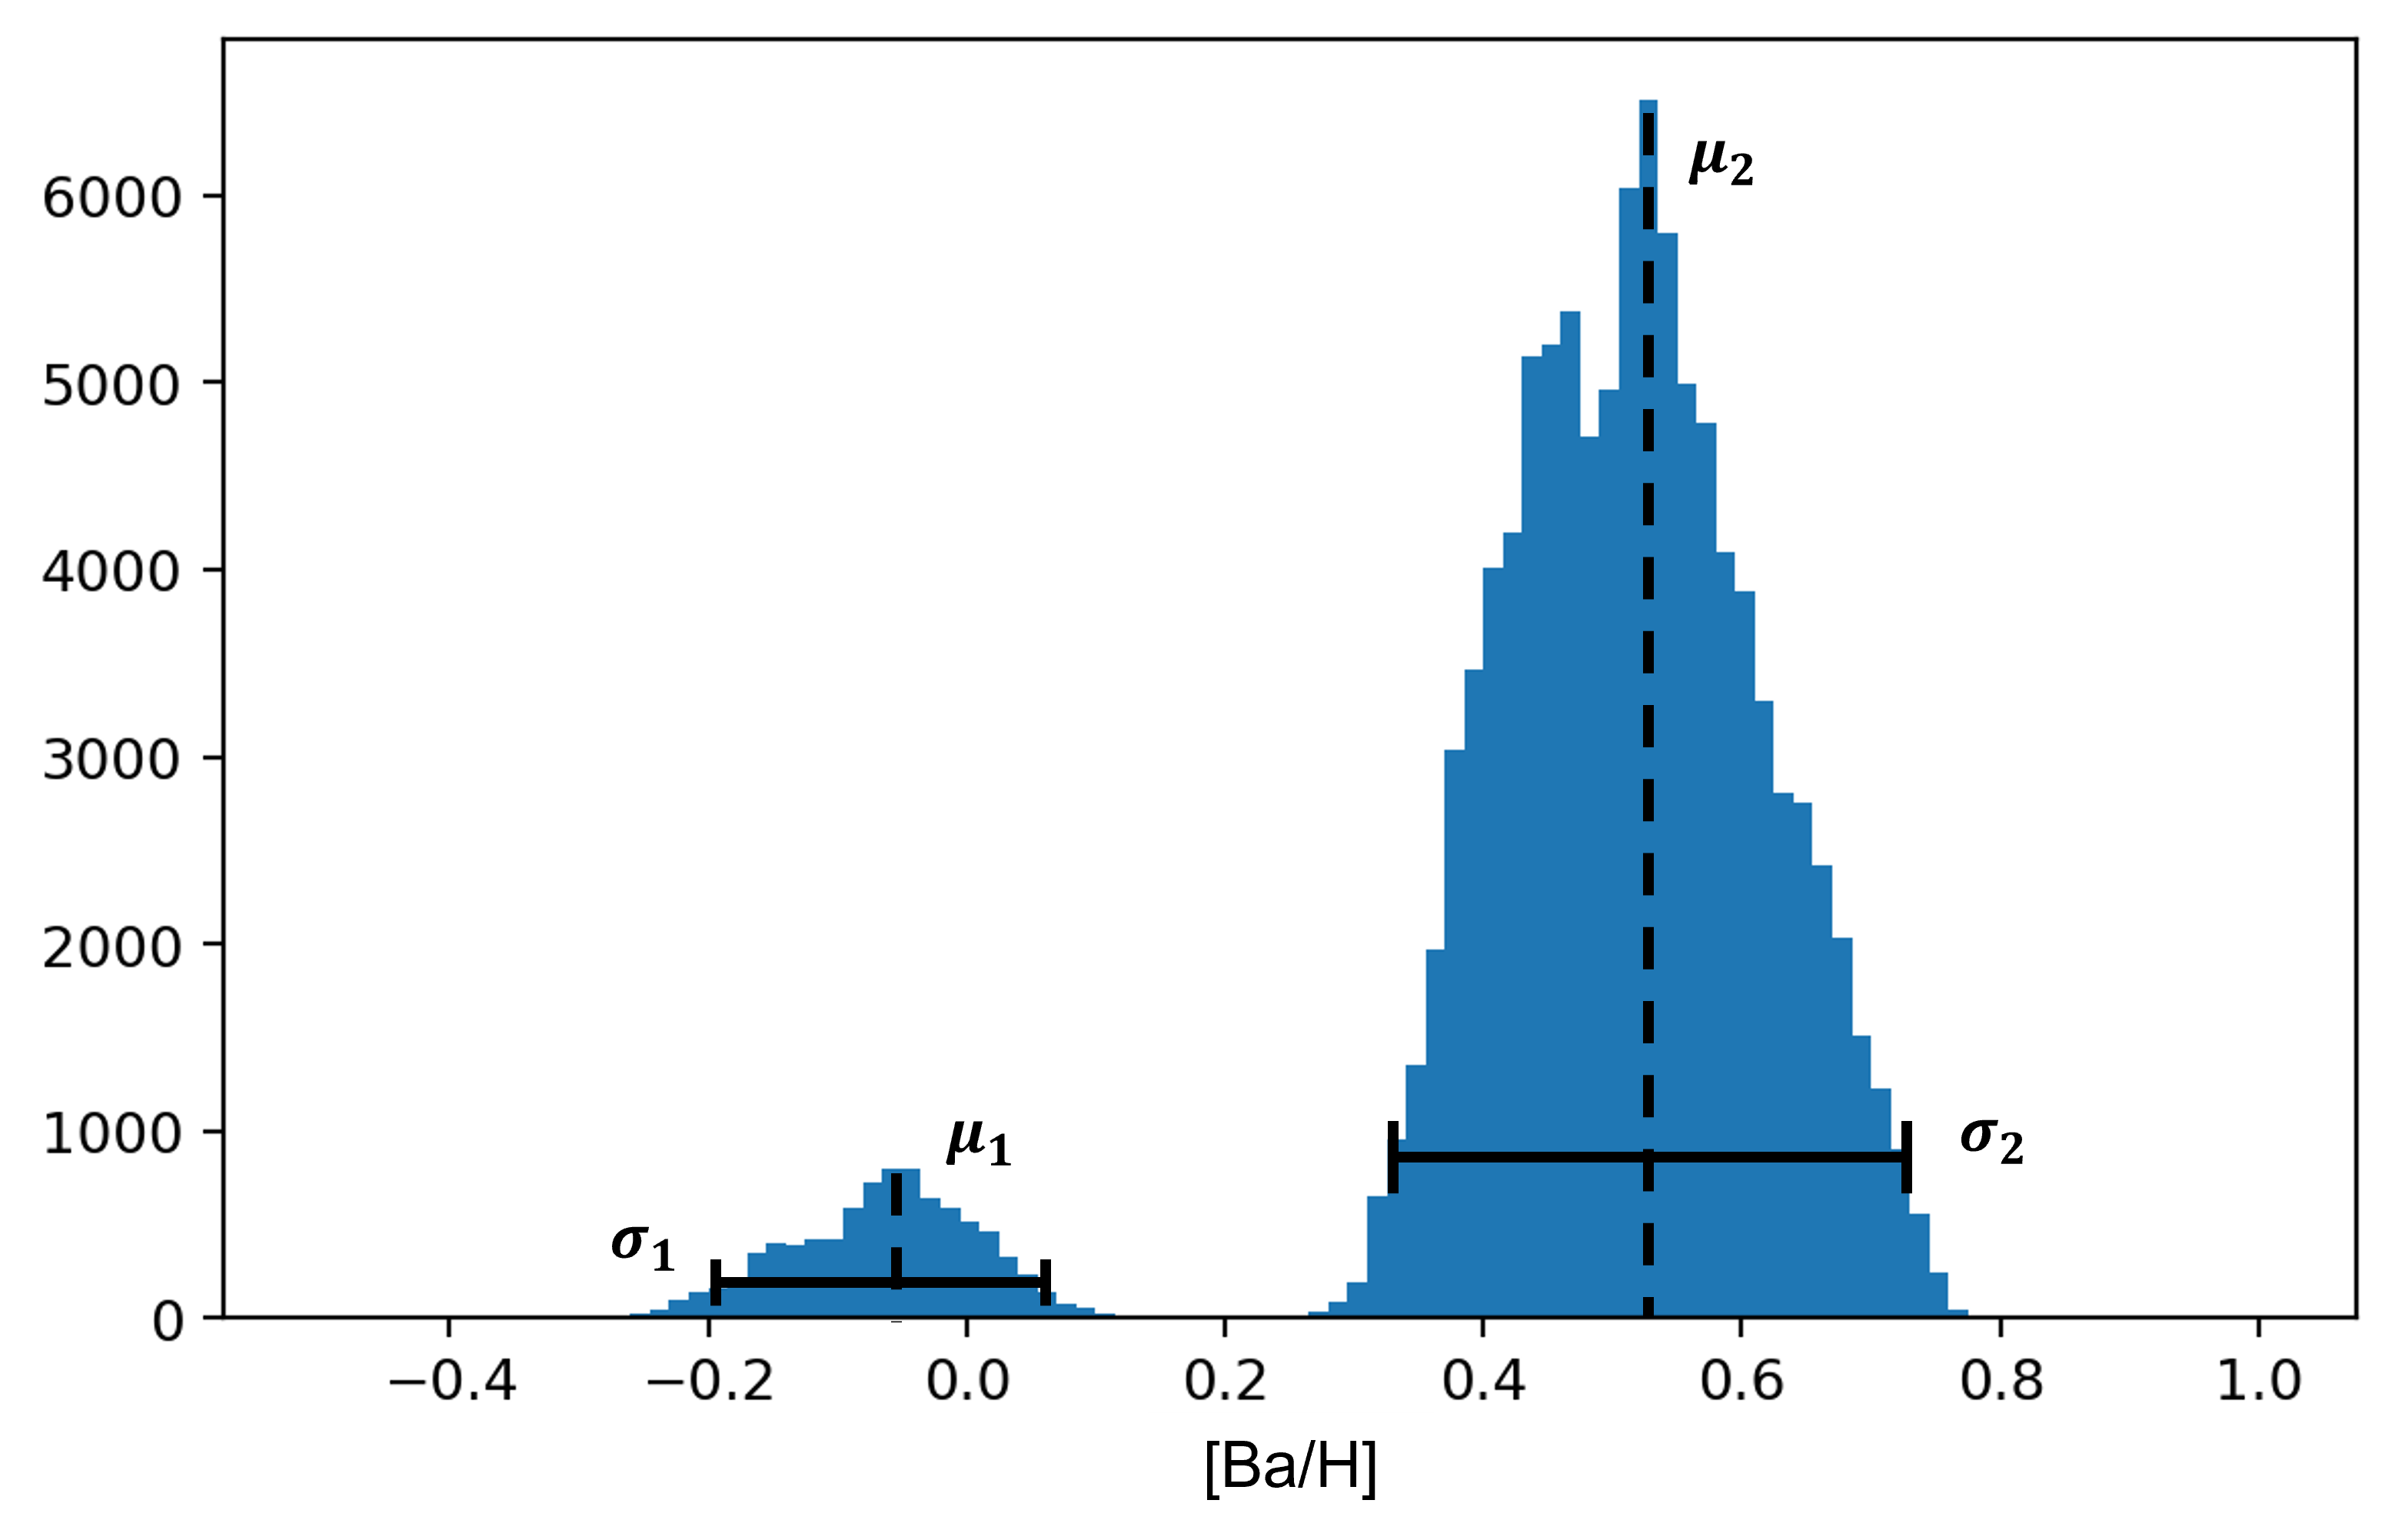
\includegraphics[width=\columnwidth]{figures/hist_labelled.png}
    \caption{A discrete 1D histogram of Barium (used just as an example), with two distinct Gaussian distributions representative of the accreted and in situ populations. This plot has been labelled with diagramatic indicators of the values of mean ($\mu_1$ and $\mu_2$) and standard deviation ($\sigma_1$ and $\sigma_2$) which are used in this project to quantify the separation between populations.}
    \label{fig:hist_labels}
\end{figure}

Fig.~\ref{fig:hist_labels} is a visual representation of the two populations we are working with limted to the ages of $8-9\,\mathrm{Gyr}$. The larger peak represents the in-situ population (also the higher 'stream' in Fig.~\ref{fig:BaHtime}). Assuming a Gaussian distribution, we determine the values of $\mu_1$, $\mu_2$, $\sigma_1$ and $\sigma_2$, which can be used to calculate the separation significance according to Eq.~\ref{eq:r_value}. These values are all displayed in Table.~\ref{tab:r_values_simulation}
\LM{Should $\mu_1$ etc. be labelled $\mu_{acc}$ etc. instead?}

To determine the positions of the sequences and subsequent separation of data to calculate $\mu_1$ and $\mu_2$, we estimated the mean [X/H] values for in-situ and accreted stars at the ages of $8-9\,\mathrm{Gyr}$. This was done visually, through looking at the histogram of each element as in Fig.~\ref{fig:hist_labels} and setting an upper and lower limit for each sequence. \SB{Need to make this more quantitative via Python.}

We then split the dataset for this particular into 2 and calculated 16th, 50th, and 84th percentiles in order to recover a more robust mean and standard deviation (and monitor our assumption of a Gaussian distribution).
\SB{We list the values of 16th, 50th, and 84th percentiles as well as the resulting $r$ values in Tab.~\ref{tab:r_values_simulation}.}

\begin{table}
    \centering
    \caption{Separation significance for the simulated data between in-situ and accreted (accr.) sequences for abundances ratios [X/H] of ten elements X.}
    \begin{tabular}{cccccc}
    \hline
    Element & $\mu_\text{in-situ}$ & $\sigma_\text{in-situ}$ & $\mu_\text{accr.}$ & $\sigma_\text{accr.}$ & $r$\\
    \hline \hline
    {[C/H]}  & 0.0 & 1.0 & 0.0 & 1.0 & 5.3 \\
    {[O/H]}  & 0.0 & 1.0 & 0.0 & 1.0 & 5.3 \\
    {[Mg/H]}  & 0.0 & 1.0 & 0.0 & 1.0 & 5.3 \\
    \hline
    \end{tabular}
    \label{tab:r_values_simulation}
\end{table}


\subsection{Assessing the influence of observational uncertainties}

\begin{itemize}
    \item abundances uncertainties, entering as $\sigma_{\text{obs}}$ into Eq.~\ref{eq:r_value_observed}.
    \item age uncertainties, making it hard to distinguish between the sequences for the oldest stars.
\end{itemize}

Assessing both influences in the observational data is difficult because we do not know the underlying distribution of accreted versus in-situ stars. We therefore turn to the simulations and perform two tests. Firstly, we test how much observational scatter $\sigma_{\text{obs}}$ is allowed to still tell apart the sequences with a confidence of 68 or 95\% ($r$-values of at least 1 or 2)? Secondly, we test how well we can tell the sequences apart when adding age uncertainties. In this particular case, we start from our initial subset selected for ages of $8-9\,\mathrm{Gyr}$ and ask, how would our selection change, if we cannot separate these stars from the even older ones (increasing our selection from $8-9\,\mathrm{Gyr}$ towards $8-10\,\mathrm{Gyr}$, $8-11\,\mathrm{Gyr}$, etc.)?

We plot the results of the first test, $r (\sigma_\text{obs})$ in Fig.~\ref{fig:r_v_obs} and compare it to the average reported uncertainty from GALAH. There is very little range between elements on these plots, and it is clear that all elements require a level of noise to be below approximately 0.4 to be 68\% sure the populations are separate, and below 0.2 to be 95\% confident. Within the accessible GALAH dataset, we can access the corresponding measurement uncertainties, and find that most, but not all, measurements of chemical abundances fall below these thresholds - if they can be measured and are reported.

\begin{figure}
	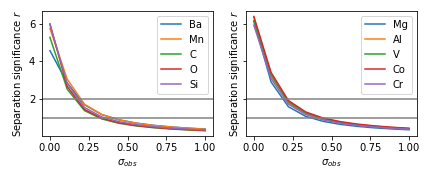
\includegraphics[width=\columnwidth]{figures/same_axis_r_sigma.png}
    \caption{Similar to Fig.~\ref{fig:r_v_age}, this plot shows all elements on an axis of their separation significance $r$ as a function of measurement noise. There are two horizontal lines at $r=1$ and $r=2$ which show the points at which we can be 68\% and 95\% confident (respectively) that we are observing two distinct populations. It is clear that these values are quite similar for all elements.}
    \label{fig:r_v_obs}
\end{figure}

\begin{table}
    \centering
    \caption{Observational uncertainties for each element that allow to separate the in-situ and accreted sequences at $8-9\,\mathrm{Gyr}$ with 95\% ($r>2$) and 68\% ($r>1$) certainty. The last rows report the percentage of measurements and their the median uncertainties for the element reported by GALAH DR3 (as indicators of how often and how well the element can be measured.}
    \begin{tabular}{ccccc}
    \hline
    Element & $\sigma_\text{obs}$ 95\% & $\sigma_\text{obs}$ 68\% & Det. Rate & $\sigma_\text{GALAH}$ \\
    \hline \hline
    {[C/H]}  & 0.132 & 0.289 & 55.8 & 0.128 \\
    {[O/H]}  & 0.158 & 0.316 & 97.35 & 0.128 \\
    {[Mg/H]}  & 0.158 & 0.342 & 100.0 & 0.078 \\
    {[Al/H]}  & 0.184 & 0.395 & 97.84 & 0.069 \\
    {[Si/H]}  & 0.158 & 0.316 & 99.57 & 0.058 \\
    {[V/H]}  & 0.184 & 0.395 & 52.3 & 0.134 \\
    {[Cr/H]}  & 0.184 & 0.368 & 98.88 & 0.077 \\
    {[Mn/H]}  & 0.184 & 0.368 & 99.66 & 0.079 \\
    {[Co/H]}  & 0.211 & 0.421 & 69.67 & 0.114 \\
    {[Ba/H]}  & 0.158 & 0.368 & 99.9 & 0.089 \\
    \hline
    \end{tabular}
    \label{tab:uncertainties}
\end{table}


\begin{figure}
	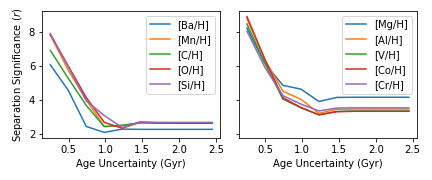
\includegraphics[width=\columnwidth]{figures/same_axis_r_age.png}
    \caption{Separation significance $r$ against age uncertainty (in Gyr) for all elements. These plots were made using data in the time-span between 4 and 5 Gyr after formation. So a 1 Gyr uncertainty is just over 20\% uncertainty. The five elements in the right-side plot have notably higher r-values than those in the left plot. The figure clearly demonstrates the age uncertainty at which we can become quite confident that we are observing two separate populations.}
    \label{fig:r_v_age}
\end{figure}

This further motivates our second test of the influences of ages. Fig.~\ref{fig:r_v_age} shows each element plotted with r-value against age uncertainty (in Gyr). These particular plots were created using data between \SB{4 and 5 Gyr - have to be adjusted to stellar age}, which means that a 1 Gyr uncertainty is equivalent to just over 20\%. From these plots, we can see that there is a fair amount of variance between the elements. Regardless, it is clear that at an uncertainty of around 1.25 Gyr (or 25\%) the r-value begins to increase. At the next interval of around 0.75 Gyr (or 15\%) there is a very rapid increase in confidence. This informs us that ideally, we are striving for an uncertainty of less than 15\%, which is significantly lower than the uncertainties we are working with at the moment.

\SB{I believe we should rather perform some MC simulations of relative abundance and age uncertainties. We can do that quite simple by multiplying the ages by a factor that is sampled from a normal distribution around 1 with a scatter value, e.g. 0.15 - is 0.15 corresponding to 15\% uncertainty?}

\subsection{}

\begin{figure}
	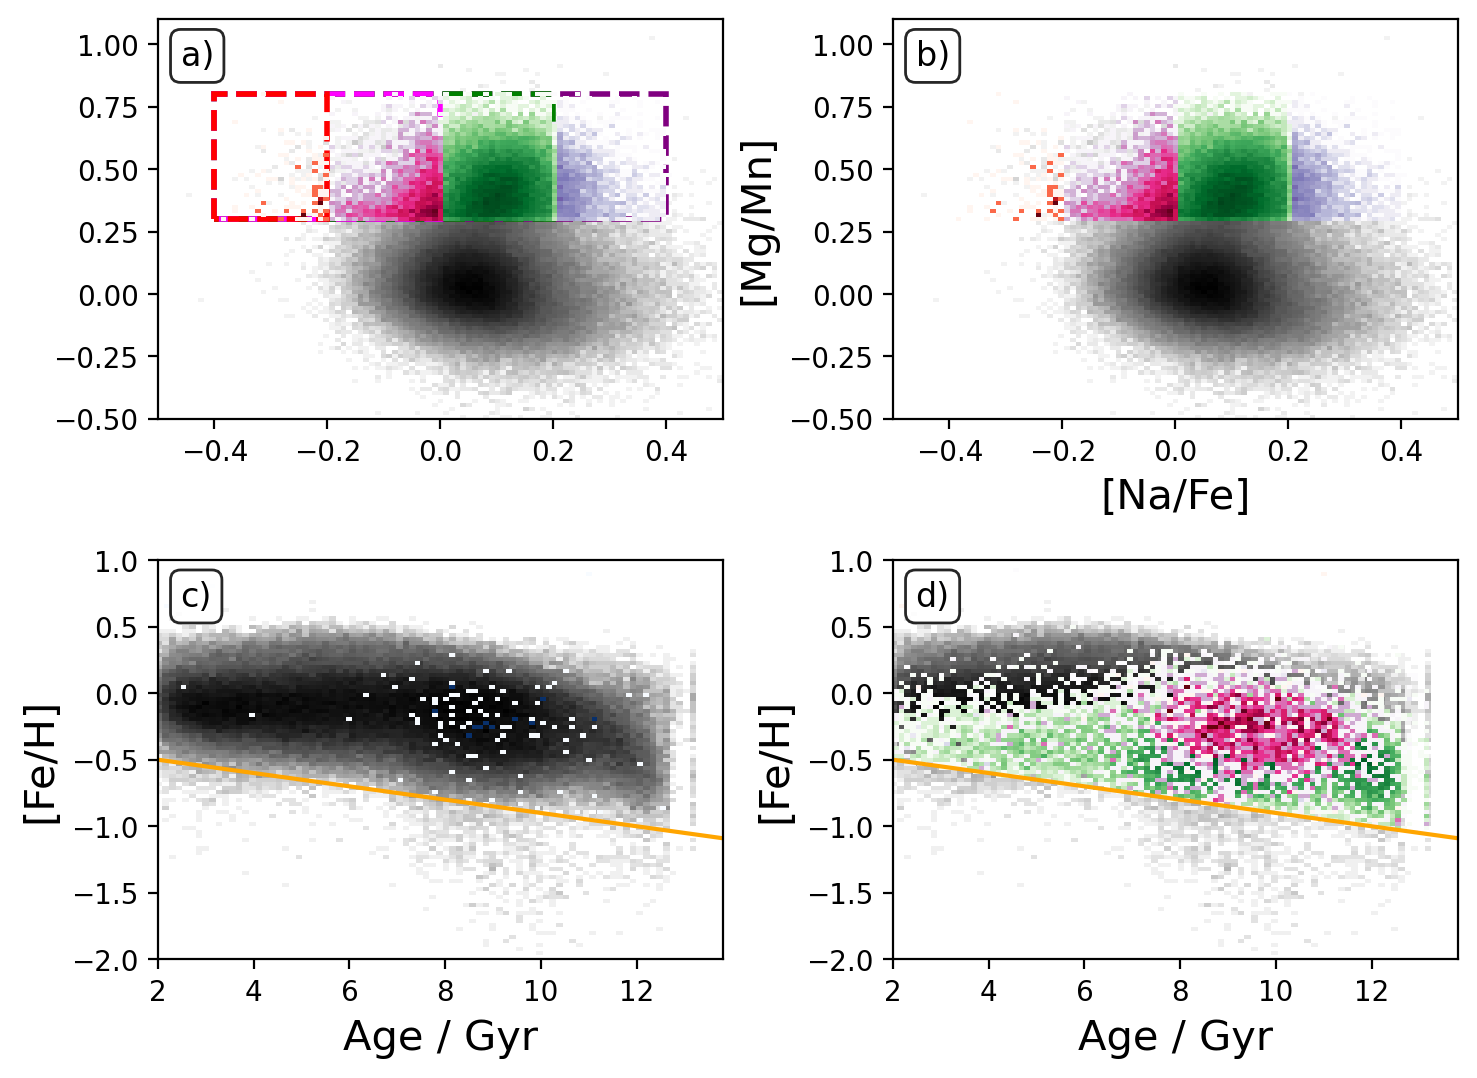
\includegraphics[width=\columnwidth]{figures/NaFe_MgMn_selection_Age_FeH_dissection.png}
    \caption{Different selections of accreted stars and how they appear in the age-xh diagram.}
    \label{fig:NaFe_MgMn_selection_Age_FeH_dissection}
\end{figure}

%%%%%%%%%%%%%%%%%%%%%%%%%%%%%%%%%%%%%%%%%%%%%%%%%%
\section{Discussion} \label{sec:discussion}

This project began with the intention of creating a variety of abundance planes and comparing both simulation and observation data to identify substructure within the plots that was representative of accreted stars. Upon doing so, and observing very little clear substructure in the simulation plots, these plots were deemed insufficient to confidently report any results. There are two major advantages to using cosmological simulations. The first of these is that there are no measurement uncertainties to consider, which should produce clear and accurate plots with no doubt of extrinsic scatter. This means that although some distinct populations were seen in the observational plots, the absence of clarity in the simulation-based plots questions that measurement uncertainties are the main difference between observations and simulations.   
Beyond measurement uncertainties, the second key advantage to the cosmological simulations is that the exact, detailed formation history of the simulated galaxy is known. Knowing what merged with the galaxy and when is crucial in identifying accretion, but this is knowledge that we don't possess to a desirable level for the Milky Way in reality. This poses a challenge in how we can use the cosmological simulations, as we have no guarantee that we are simulating the evolution of the Milky Way. It may also contribute to the discrepancies between the simulations and observations. If the simulations are replicating even a slightly different galaxy, this could explain the lack of clear substructure that we can see in observations. We know that the simulations are based on a merger event that occurred 5Gyr after formation, when a galaxy around $10^9 M_{\odot}$ merged with an in situ galaxy of around $10^{10} M_{\odot}$, values that have been estimated to the order of magnitude by multiplying the number of star particles with their average stellar mass for each sequence of the simulation. Although we do not know the exact sizes or times of accretion events in the Milky Way, the GSE is estimated to be between $10^{8.7}$ and $10^{9.85}\,M_{\odot}$ \citep{Helmi2018,Naidu2020}, which highlights a possible discrepancy between the simulations and the observations. Until we have a more exact understanding of the formation history of the Milky Way, we cannot ensure these simulations are accurate, which is an important caveat to keep in mind.   
From this, the focus of the project underwent a shift, looking instead at other observables beyond chemical abundance that could be used and plotted to identify accreted stars. As Section \ref{sec:intro} makes clear, one of the key advantages to chemical tagging is the unchanging nature of stellar chemistry over time, meaning that a star's current chemical make-up is indicative of the time and place that it was born. Therefore, plotting elemental abundance over time was hypothesised as a good indicator of accretion, where separate populations should be clear. This was plotted and analysed in Section \ref{sec:ageabundance}, and found that indeed there are two clear stellar populations in the simulation data, indicative of accreted and in situ stars, that were not seen in the observational data due to measurement uncertainties.  
Despite this positive outcome, it is still important to address the possibility of intrinsic overlap between accreted and in situ stars. As discussed, there are two clear streams that have been attributed as accreted and in situ, based on the assumption that the accreted stars would have been born in a smaller galaxy with less massive stars and therefore lower element abundances. This clarity occurs because we know the sizes of the two galaxies that merged. Depending on the size of the real merger in the Milky Way, there could be significantly more overlap between the accreted and in situ populations if the merger was more massive. This means that from the abundance-age plots alone, it is harder to tell if the situ stream is completely made up of Milky Way-born stars. 

A further recommendation is that it would be worth putting effort into further analysing Fig.~\ref{fig:BaHtime}. Despite the massive amount of scatter in the observations, when Ba was plotted in a ratio with H, there appears to be a hint of an overdensity toward the bottom right of the plot, which could indicate an accreted population. Applying the quality cuts provided in the GALAH data had little effect on how clear this overdensity appears. It is beyond the scope of this project, but with better quality cuts, more time and expertise - and better data, this 'hint' could start indicating something that looks more like the simulations, which would further confirm that plots of elements against time are worth pursuing.  
This project was limited by a number of variables, one of which was simply the number of elements that could be analysed. The caveat for an element to be used in this project was that it had to be included in the datasets of both the simulations, and the GALAH survey. This reduced the total number of elements to just ten. Moreover, although there were quite a number of iron-peak elements, the remaining element groups only contained two options, with Ba being the only neutron capture element. This reduced the ability to make in-depth assessments based on element groups, as the sample size was simply not large enough to consider any trends with certainty. To this end, it could be worth pursuing other datasets with a different choice of elements.  
Moreover, I would strongly recommend similar research is performed with other cosmological simulations, preferably with varied chemistry and formation histories. This would enable researchers to observe exactly how different variables in the simulation affect outcomes. 
The main observational limitation to this project was simply measurement uncertainties, particularly in ages. If the errors corresponding to age measurements can be drastically reduced, plotting elements over time has the potential to be a great diagnostic tool for accreted stars. 


%%%%%%%%%%%%%%%%%%%%%%%%%%%%%%%%%%%%%%%%%%%%%%%%%%

%%%%%%%%%%%%%%%%%%%%%%%%%%%%%%%%%%%%%%%%%%%%%%%%%%
\section{Conclusions}
\label{sec:conc}

The aim of this project was to determine suitable diagnostic plots for identifying accreted stars in our Milky Way, through comparison of a cosmological simulation from the NIHAO suite with data from the GALAH survey. The major take-aways from this undertaking were:
\begin{itemize}
\item Chemical abundance planes of the simulations possess too much intrinsic overlap to be useful to this particular research project. 
\item Plotting elemental abundances against age however, proved fruitful, with very distinct streams representing accreted and in situ populations appearing in the simulation data. These clear streams were not apparent in the observation-based plots, as a result of massive uncertainties that come with the probabilistic nature of estimating stellar ages through isochrone fitting.
\item Elemental abundances as relative to H (rather than Fe) produced more significant separations between in-situ and accreted sequences as a function of stellar age.
\item Our tests of adding noise to simulated data suggest, that we will be able to more easily tell apart accreted structures, once we undergo a critical age uncertainty of 15\% and can measure elemental abundances [X/H] of accreted structures as good as $\sigma_\text{obs} \sim 0.40\,\mathrm{dex}$.
\end{itemize}

Overall, reducing uncertainties in ages is a difficult task that may take a long time, but as data and techniques continue to improve these values, there is much potential in using plots of elemental abundances over time as a diagnostic tool for accreted stars.

\section*{Acknowledgements}

We acknowledge the traditional owners of the land on which the AAT and ANU stand, the Gamilaraay, the Ngunnawal and Ngambri people. We pay our respects to elders past, present, and emerging and are proud to continue their tradition of surveying the night sky in the Southern hemisphere.

This work was supported by the Australian Research Council Centre of Excellence for All Sky Astrophysics in 3 Dimensions (ASTRO 3D), through project number CE170100013.

TB acknowledges support from the European Research Council under ERC-CoG grant CRAGSMAN-646955.

\section*{Facilities}

\textbf{AAT with 2df-HERMES at Siding Spring Observatory:}
The GALAH Survey is based data acquired through the Australian Astronomical Observatory, under programs: A/2013B/13 (The GALAH pilot survey); A/2014A/25, A/2015A/19, A2017A/18 (The GALAH survey phase 1), A2018 A/18 (Open clusters with HERMES), A2019A/1 (Hierarchical star formation in Ori OB1), A2019A/15 (The GALAH survey phase 2), A/2015B/19, A/2016A/22, A/2016B/10, A/2017B/16, A/2018B/15 (The HERMES-TESS program), and A/2015A/3, A/2015B/1, A/2015B/19, A/2016A/22, A/2016B/12, A/2017A/14, (The HERMES K2-follow-up program). This paper includes data that has been provided by AAO Data Central (datacentral.aao.gov.au).

\textbf{\Gaia: } This work has made use of data from the European Space Agency (ESA) mission \Gaia (\url{http://www.cosmos.esa.int/gaia}), processed by the \Gaia Data Processing and Analysis Consortium (DPAC, \url{http://www.cosmos.esa.int/web/gaia/dpac/consortium}). Funding for the DPAC has been provided by national institutions, in particular the institutions participating in the \Gaia Multilateral Agreement. 

\textbf{Other facilities:} This publication makes use of data products from the Two Micron All Sky Survey \citep{Skrutskie2006} and the CDS VizieR catalogue access tool \citep{Vizier2000}.

\section*{Software}

The research for this publication was coded in \textsc{python} (version 3.7.4) and included its packages
\textsc{astropy} \citep[v. 3.2.2;][]{Robitaille2013,PriceWhelan2018},
\textsc{corner} \citep[v. 2.0.1;][]{corner},
\textsc{IPython} \citep[v. 7.8.0;][]{ipython},
\textsc{matplotlib} \citep[v. 3.1.3;][]{matplotlib},
\textsc{NumPy} \citep[v. 1.17.2;][]{numpy},
\textsc{pynbody} \citep[v. 1.1.0;][]{pynbody},
\textsc{scipy} \citep[version 1.3.1;][]{scipy},
\textsc{sklearn} \citep[v. 0.21.3;][]{scikit-learn},
We further made use of \textsc{topcat} \citep[version 4.7;][]{Taylor2005};

%%%%%%%%%%%%%%%%%%%%%%%%%%%%%%%%%%%%%%%%%%%%%%%%%
\section*{Data Availability}

The observational data used for this study is published by \citet{Buder2021} and can be accessed publicly via \url{https://docs.datacentral.org.au/galah/dr3/overview/}

All code to reproduce the analysis and figures can be accessed via \url{https://github.com/svenbuder/Accretion_Clues_ObsSim}.

Simulated data can be retrieved from the authors upon reasonable request.

%%%%%%%%%%%%%%%%%%%% REFERENCES %%%%%%%%%%%%%%%%%%

% The best way to enter references is to use BibTeX:
\bibliographystyle{mnras}
\bibliography{bib} % if your bibtex file is called example.bib

%%%%%%%%%%%%%%%%%%%%%%%%%%%%%%%%%%%%%%%%%%%%%%%%%%
%%%%%%%%%%%%%%%%% APPENDICES %%%%%%%%%%%%%%%%%%%%%

% \newpage
% \appendix

%%%%%%%%%%%%%%%%%%%%%%%%%%%%%%%%%%%%%%%%%%%%%%%%%%

% Don't change these lines
\bsp	% typesetting comment
\label{lastpage}
\end{document}

% End of mnras_template.tex
